%%%%%%%%%%%%%%%%%%%%%%%%%%%%%%%%%%%% Chapter 

\chapter{Etudes Complémentaires} 	
\label{Chapter4} 		

%%%%%%%%%%%%%%%%%%%%%%%%%%%%%%%%%%%%

%%%%%%%%%%%%%%%%%%%%%%%%%%%%%%%%%%%%%%%%%%%%%%%%%%%%%%%%%%%%%%%%%%%%%%%%%%%%%%%%
%%%%%%%%%%%%%%%%%%%%%%%%%%%%%%%%%%%% SECTION 1 %%%%%%%%%%%%%%%%%%%%%%%%%%%%%%%%%
%%%%%%%%%%%%%%%%%%%%%%%%%%%%%%%%%%%%%%%%%%%%%%%%%%%%%%%%%%%%%%%%%%%%%%%%%%%%%%%%

\section{Etude de la position de la cambrure maximale}
\label{sec:Ch4.1}

Tout d'abord Breukels ne prend en compte que le diamètre et la cambrure maximal d'un profil, \textbf{la position de la cambrure maximale d'un profil n'est donc pas prise en compte}. \\
En conduisant des simulations (VSM) basées cette fois sur des polaires déterminées à partir de NeuralFoil (Aersoandbox), on pense alors capturer l'influence de la position de la cambrure maximale. \textbf{On mène l'étude  sur des SK50-VG avec (t,k)=(0.06, 0.08)} :

\begin{figure}[H]
    \centering
    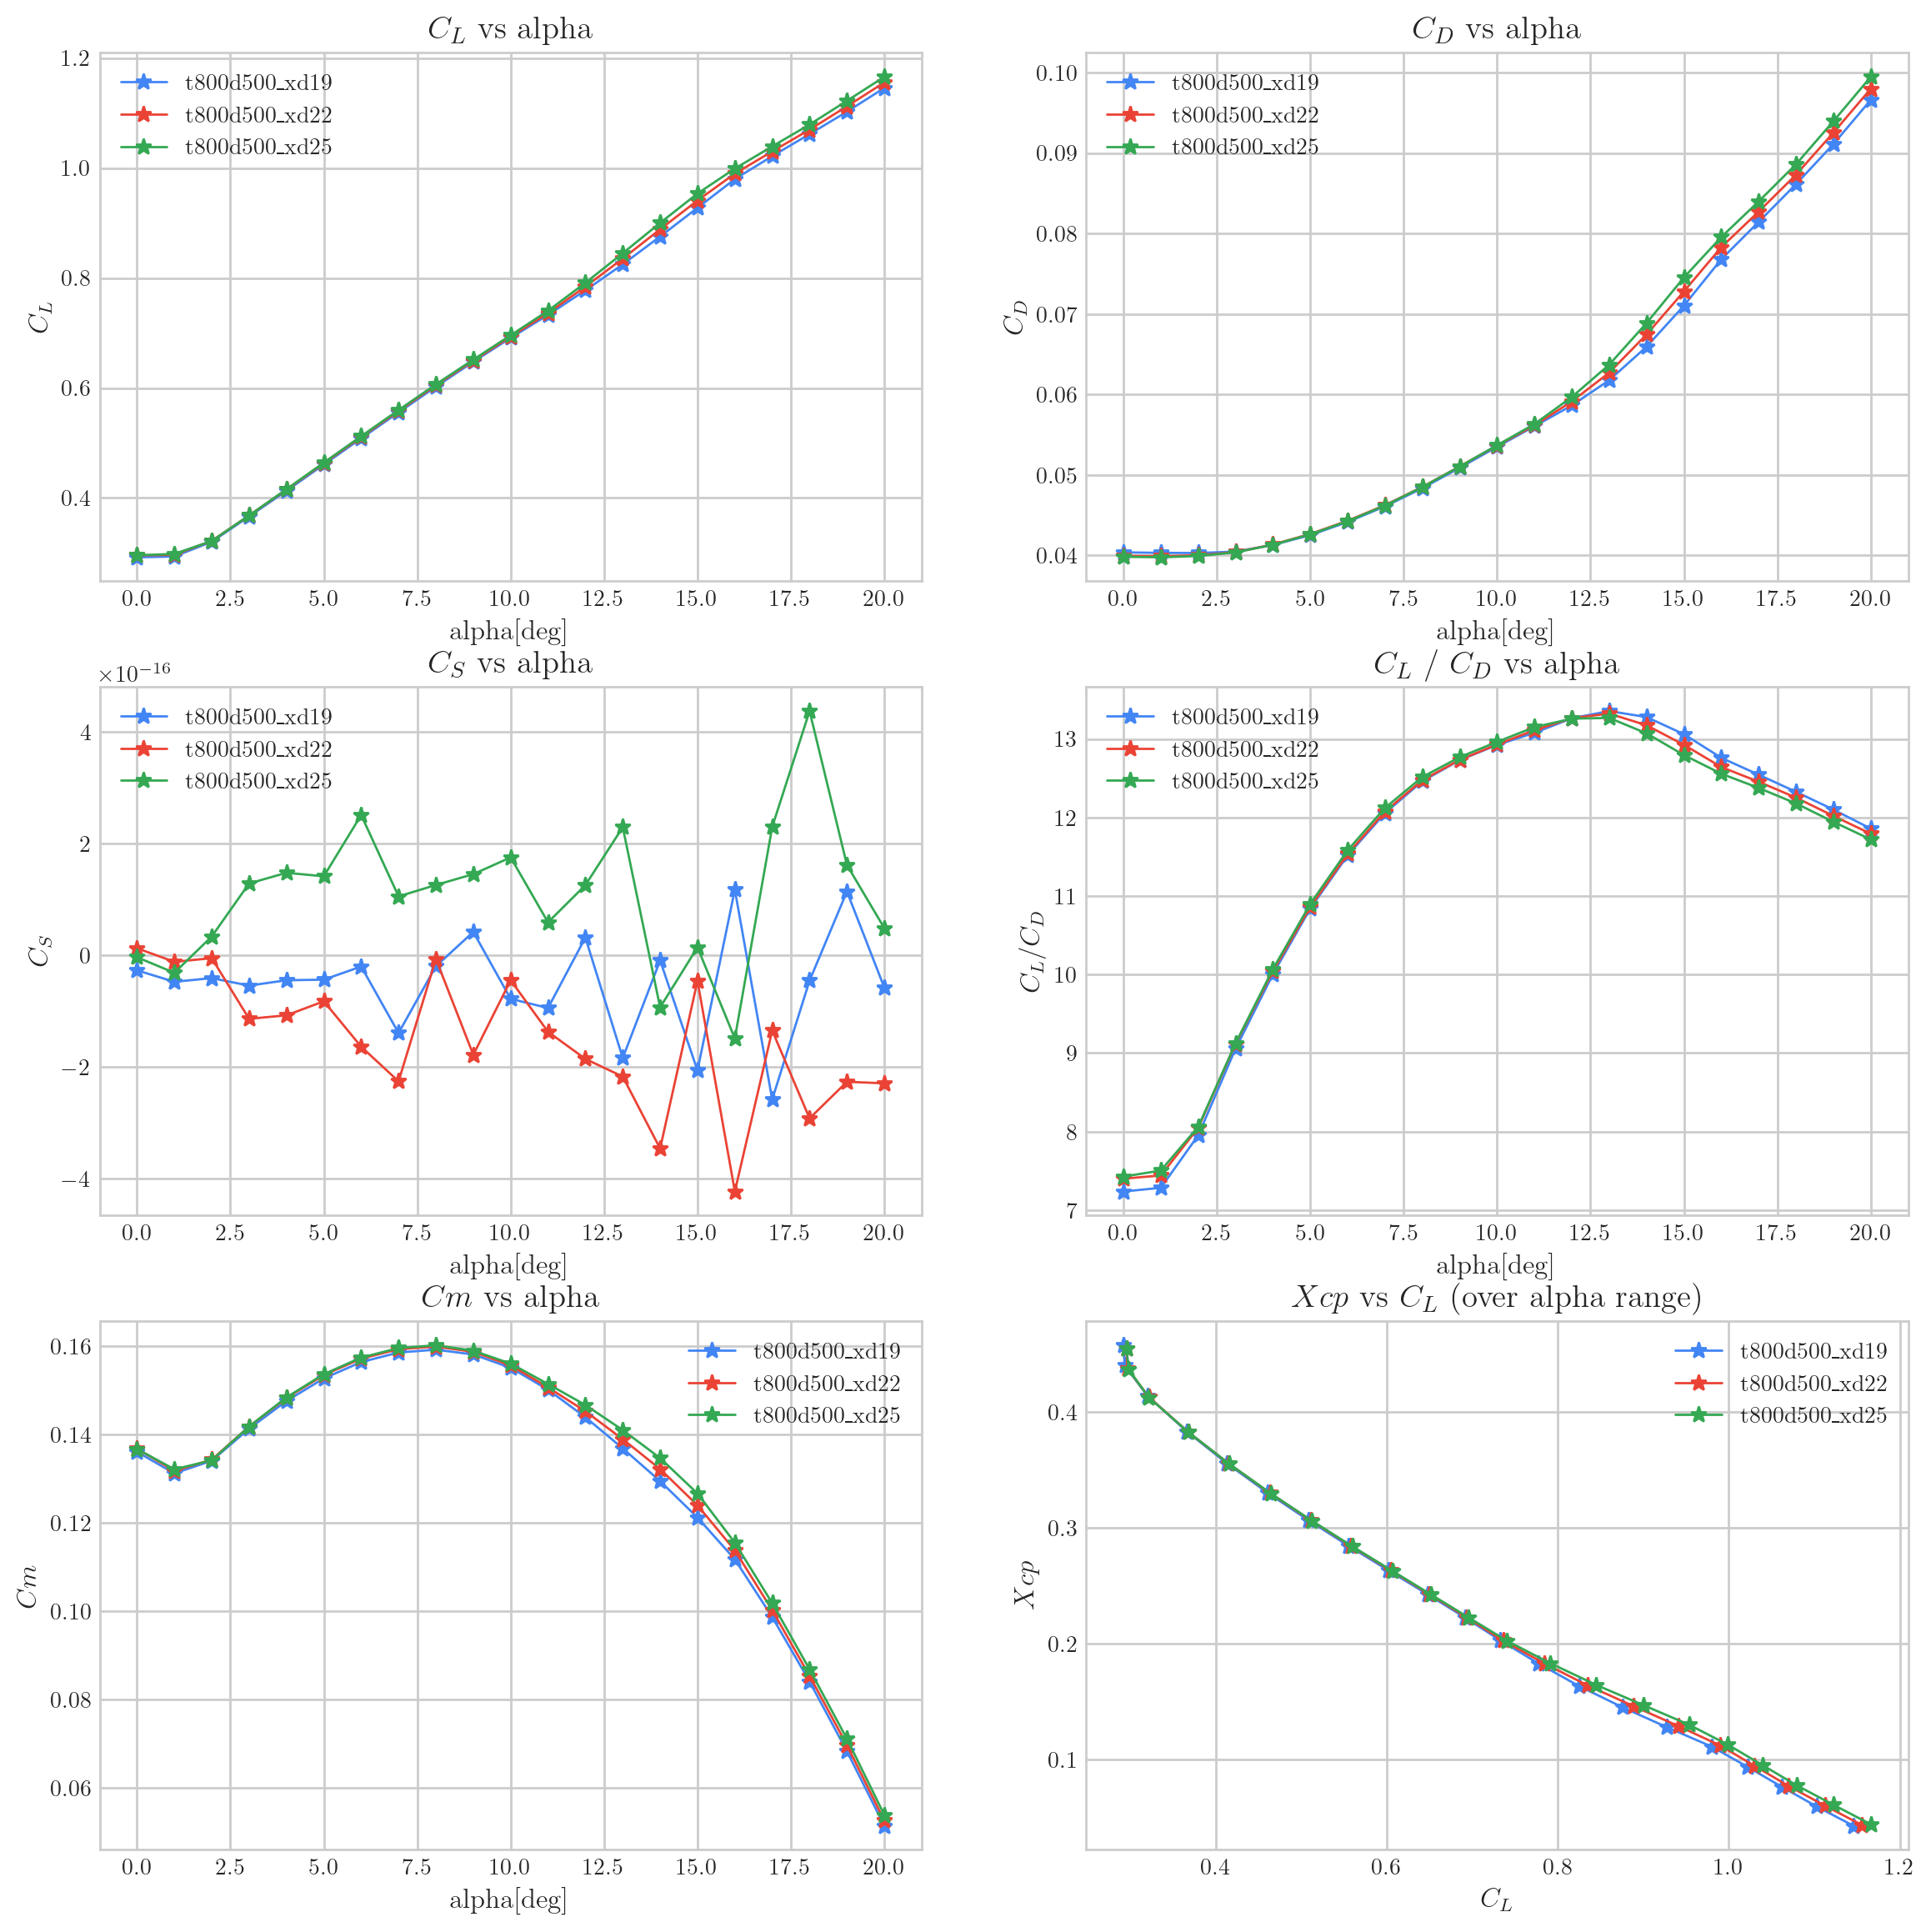
\includegraphics[width=\textwidth]{Pics/04 -Etudes complémentaires/position cambrure.png}  
    \caption{Influence de la position de la cambrure maximale}
    \label{fig:influence cambrure position}
\end{figure}

On observe que les résultats sont sensiblement les mêmes à des angles inférieurs à 10°. Cependant au delà de 10° NeuralFoil, qui est basé sur la même théorie que XFOIL (écoulement potentiel + équations couche limite) couplé avec de l'IA, perd en fiabilité. \\
\textbf{les résultats semblent donc être quasi-indentiques pour des variations de position de cambrure maximale entre 19\% et 25\%, aux faibles angles (<10°)}
%%%%%%%%%%%%%%%%%%%%%%%%%%%%%%%%%%%%%%%%%%%%%%%%%%%%%%%%%%%%%%%%%%%%%%%%%%%%%%%%
%%%%%%%%%%%%%%%%%%%%%%%%%%%%%%%%%%%% SECTION 2 %%%%%%%%%%%%%%%%%%%%%%%%%%%%%%%%%
%%%%%%%%%%%%%%%%%%%%%%%%%%%%%%%%%%%%%%%%%%%%%%%%%%%%%%%%%%%%%%%%%%%%%%%%%%%%%%%%

\section{Stabilité}
\label{sec:Ch4.2}

Ensuite, l'étude réalisée \textbf{ne fait pas intervenir de critère de stabilité.} En témoigne la figure \ref{fig:influence cambrure position}, nous avons ajouté l'évolution de Xcp, la position du centre de pousée le long de la corde, sur les polaires.\\
\textbf{\underline{Le raisonnement est le suivant} : "Xcp doit être suffisamment faible (effort aérodynamique proche du bord d'attaque) à faible Cl (limite de l'équilibre poids-portance) pour que le moment associé soit suffisamment cabreur et que l'aile ne tende pas à aller vers des Cl plus petits"}\\ 

\begin{figure}[H]
    \centering
    \begin{subfigure}[b]{0.45\textwidth}
        \centering
        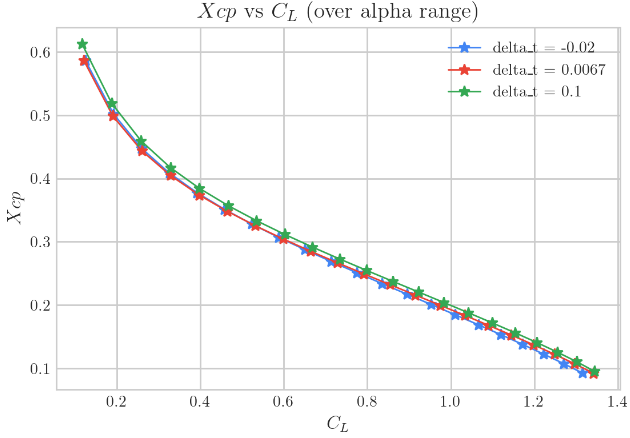
\includegraphics[width=\linewidth]{Pics/04 -Etudes complémentaires/stabilité diam.png}
        \caption{$X_{CP}$ pour différent $\delta diamètre$}
        \label{fig:stabilité diamètre}
    \end{subfigure}
    \hfill
    \begin{subfigure}[b]{0.45\textwidth}
        \centering
        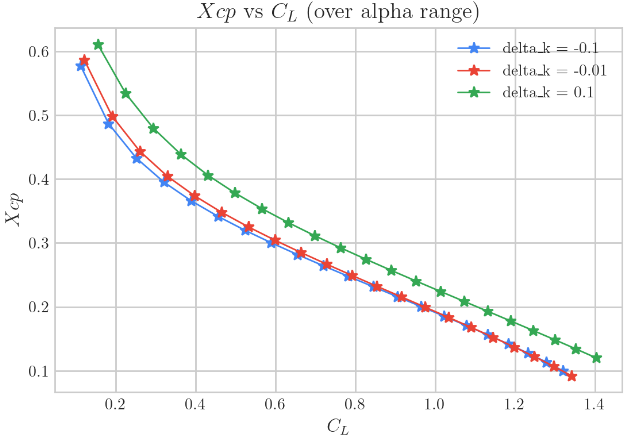
\includegraphics[width=\linewidth]{Pics/04 -Etudes complémentaires/stabilité dep.png}
        \caption{$X_{CP}$ pour différent $\delta cambrure$}
        \label{fig:stabilité cambrure}
    \end{subfigure}
    \caption{Sensibilité de la stabilité du kite aux variations de (t,k)}
    \label{fig:stabilité}
\end{figure}

Il semblerait donc que la cambrure joue un rôle majeur dans la stabilité du kite. Diminuer la cambrure déplace la courbe de $X_{CP}$ vers la gauche et donc stabilise le kite (figure \ref{fig:stabilité cambrure}). La figure \ref{fig:stabilité diamètre} montre la faible influence du diamètre de BA sur la stabilité. \\
\textbf{ Augumenter la cambrure semble donc dégrader la stabilité du kite. Ce résultat semble cohérent puisque augumenter la cambrure tend à augmenter la charge arrière. L'influence du diamètre est négligeable devant celle de la cambrure. }


%%%%%%%%%%%%%%%%%%%%%%%%%%%%%%%%%%%%%%%%%%%%%%%%%%%%%%%%%%%%%%%%%%%%%%%%%%%%%%%%
%%%%%%%%%%%%%%%%%%%%%%%%%%%%%%%%%%%% SECTION 3 %%%%%%%%%%%%%%%%%%%%%%%%%%%%%%%%%
%%%%%%%%%%%%%%%%%%%%%%%%%%%%%%%%%%%%%%%%%%%%%%%%%%%%%%%%%%%%%%%%%%%%%%%%%%%%%%%%

\section{Optimisation avec Aerosandbox}
\label{sec:Ch4.3}

Finalement les fonctions d'optimisation d'Aerosandbox ne sont pas applicables à la VSM. Elles sont cependant utilisées pour optimiser la fonction de Breukels (2 paramètres). \\
Aerosandbox peut aussi représenter et optimiser les profils avec 10 paramètres (Kulfan parameters). \textbf{Ce n'est pas le sujet de ce papier, cependant c'est une façon différente d'aborder le problème. Ce sera probablement le sujet d'une étude à venir.}

\begin{figure}[H]
    \centering
    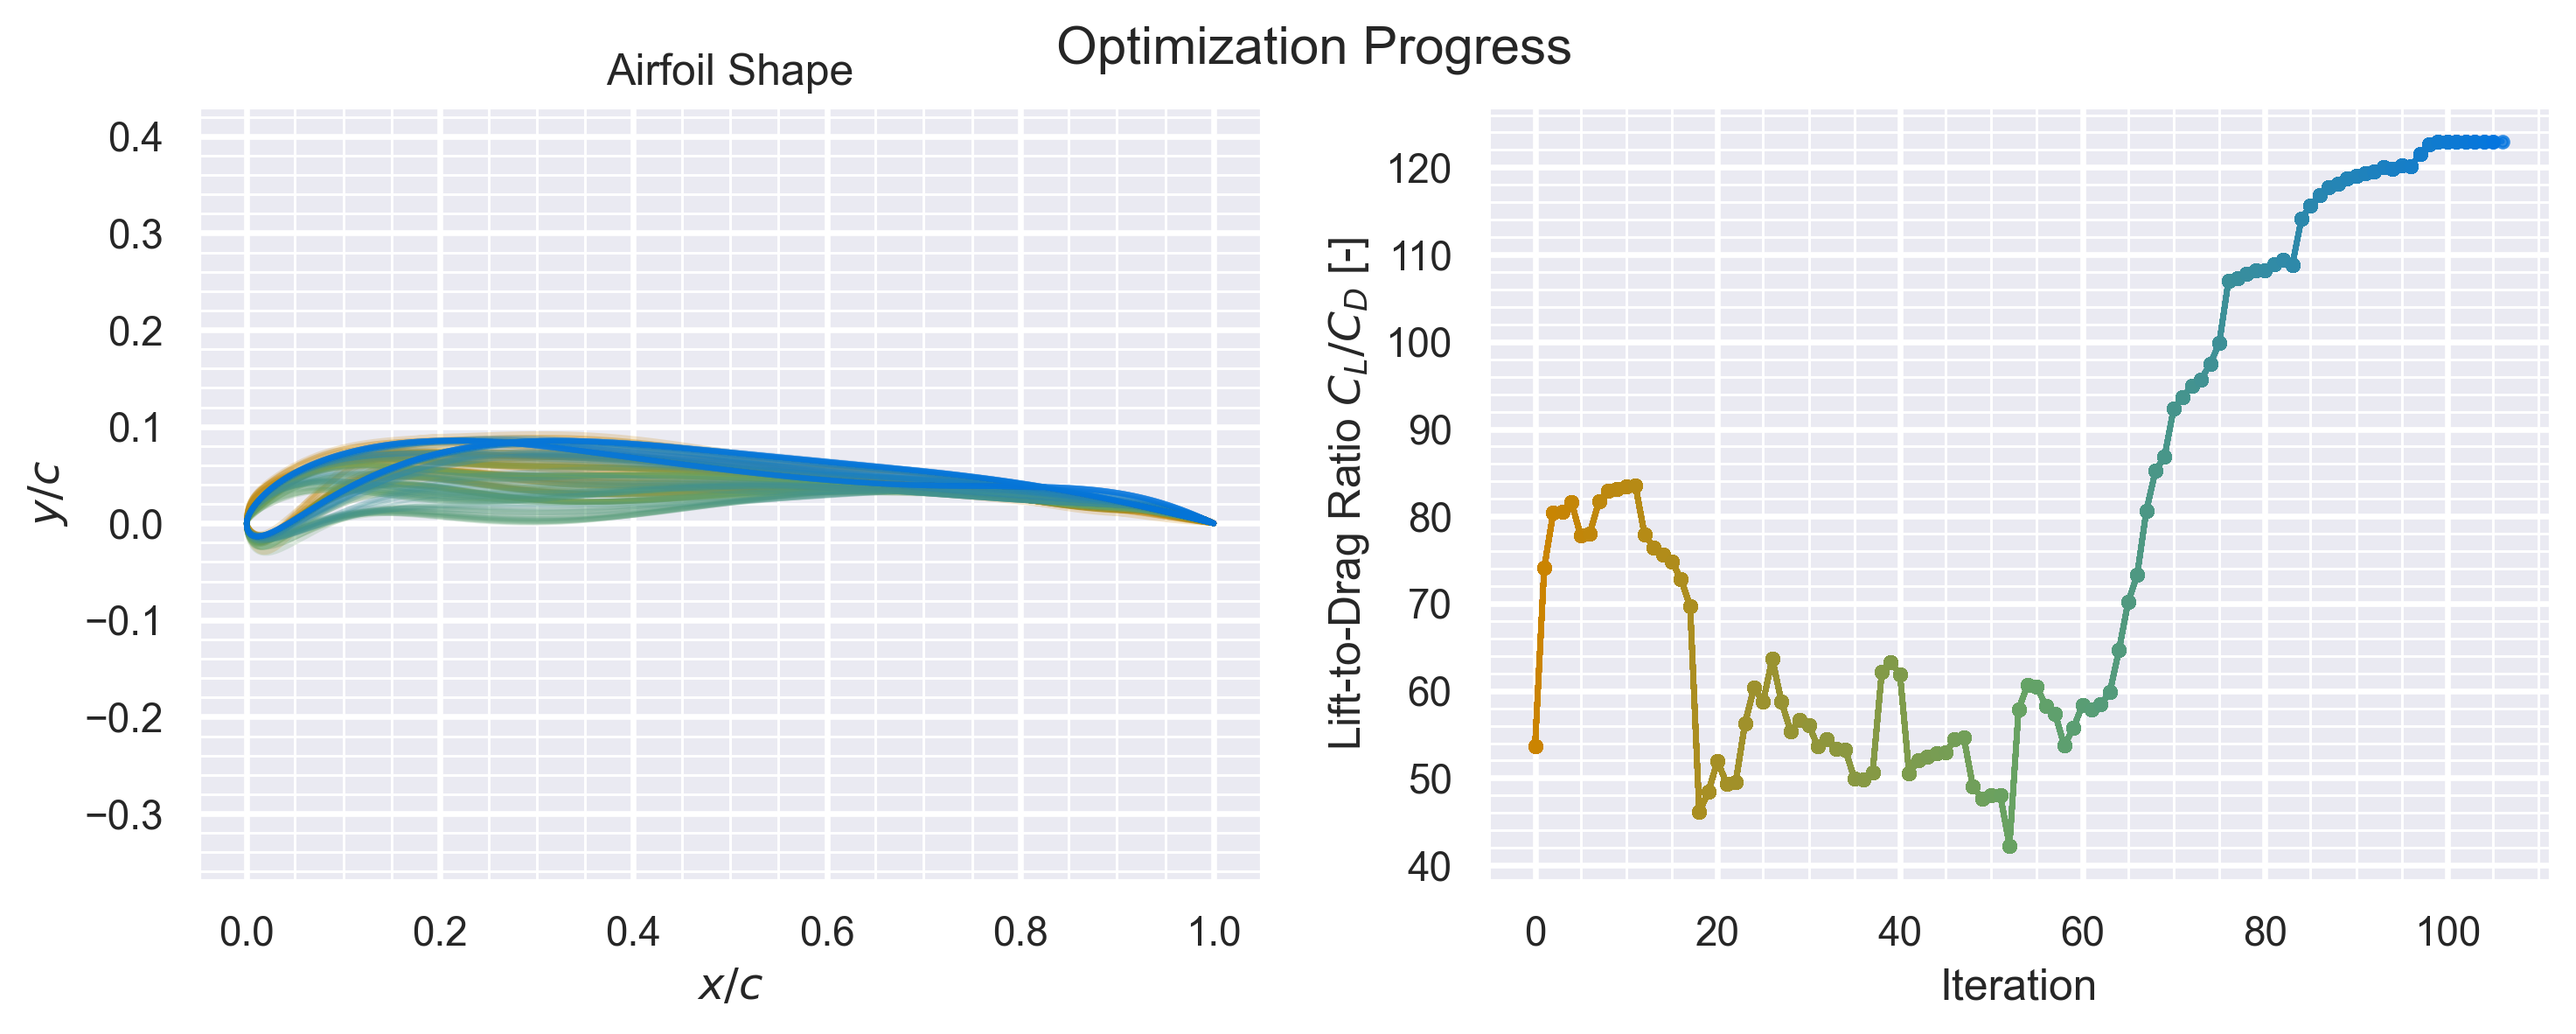
\includegraphics[width=\textwidth]{Pics/04 -Etudes complémentaires/optim neuralfoil.png}  
    \caption{Optimisation réalisée avec Aerosandbox sur des profils dis "de Kulfan"}
    \label{fig:kulfan}
\end{figure}

%%%%%%%%%%%%%%%%%%%%%%%%%%%%%%%%%%%%%%%%%%%%%%%%%%%%%%%%%%%%%%%%%%%%%%%%%%%%%%%%
%%%%%%%%%%%%%%%%%%%%%%%%%%%%%%%%%%%% SECTION 4 %%%%%%%%%%%%%%%%%%%%%%%%%%%%%%%%%
%%%%%%%%%%%%%%%%%%%%%%%%%%%%%%%%%%%%%%%%%%%%%%%%%%%%%%%%%%%%%%%%%%%%%%%%%%%%%%%%

\section{Optimisation d'un SK5}
\label{sec:Ch4.4}

La même étude que présentée dans ce papier a été réalisée sur un SK5-VB afin de permettre un premier prototype pour Beyond. Voici les résulats :\\

\begin{figure}[H]
    \centering
    \begin{subfigure}[b]{0.45\textwidth}
        \centering
        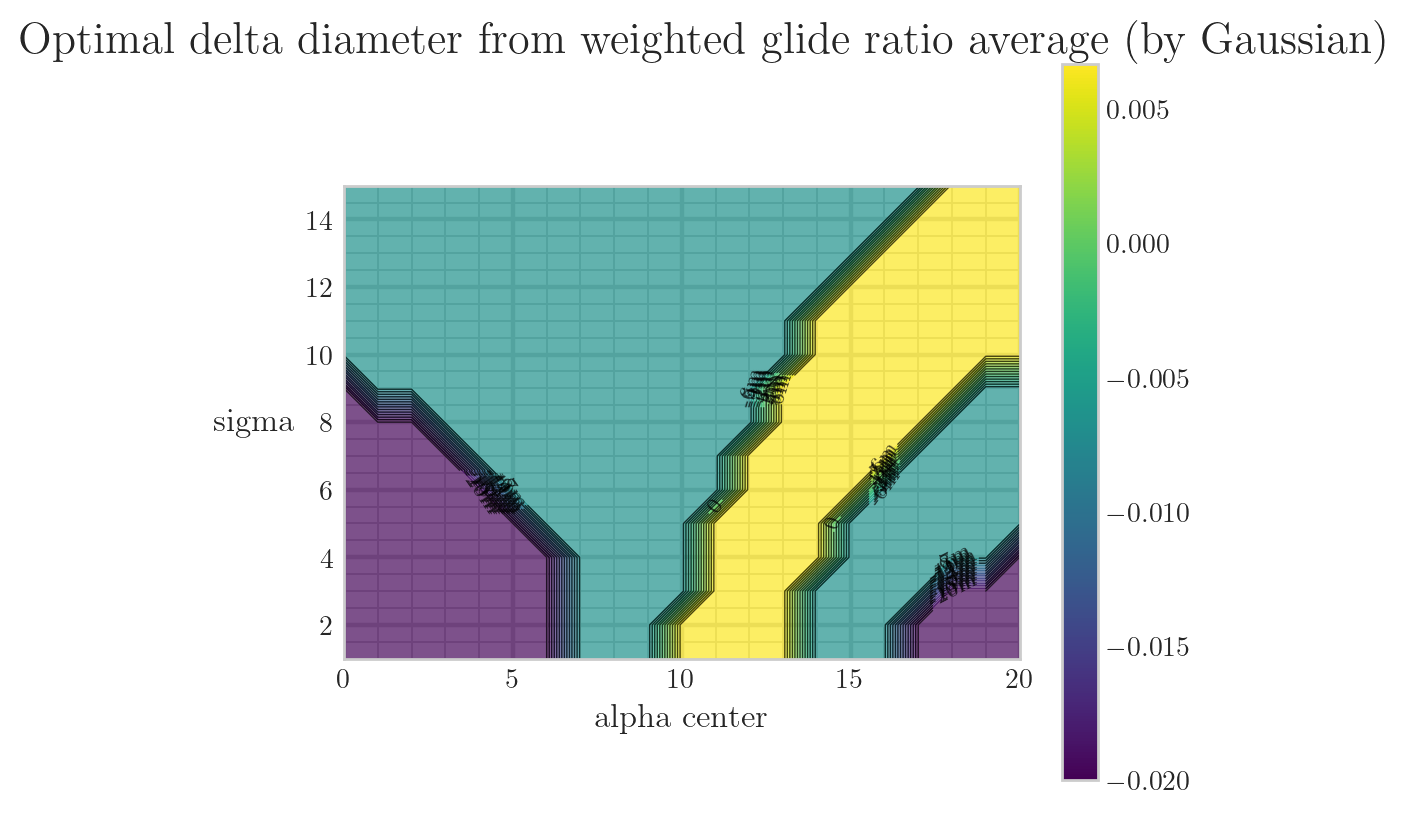
\includegraphics[width=\linewidth]{Pics/04 -Etudes complémentaires/sk5 vb guassian diameter.png}
        \caption{$\delta$ diamètre selon les paramètres de la Gaussienne}
        \label{fig:diametre gaussien sk5 vb}
    \end{subfigure}
    \hfill
    \begin{subfigure}[b]{0.45\textwidth}
        \centering
        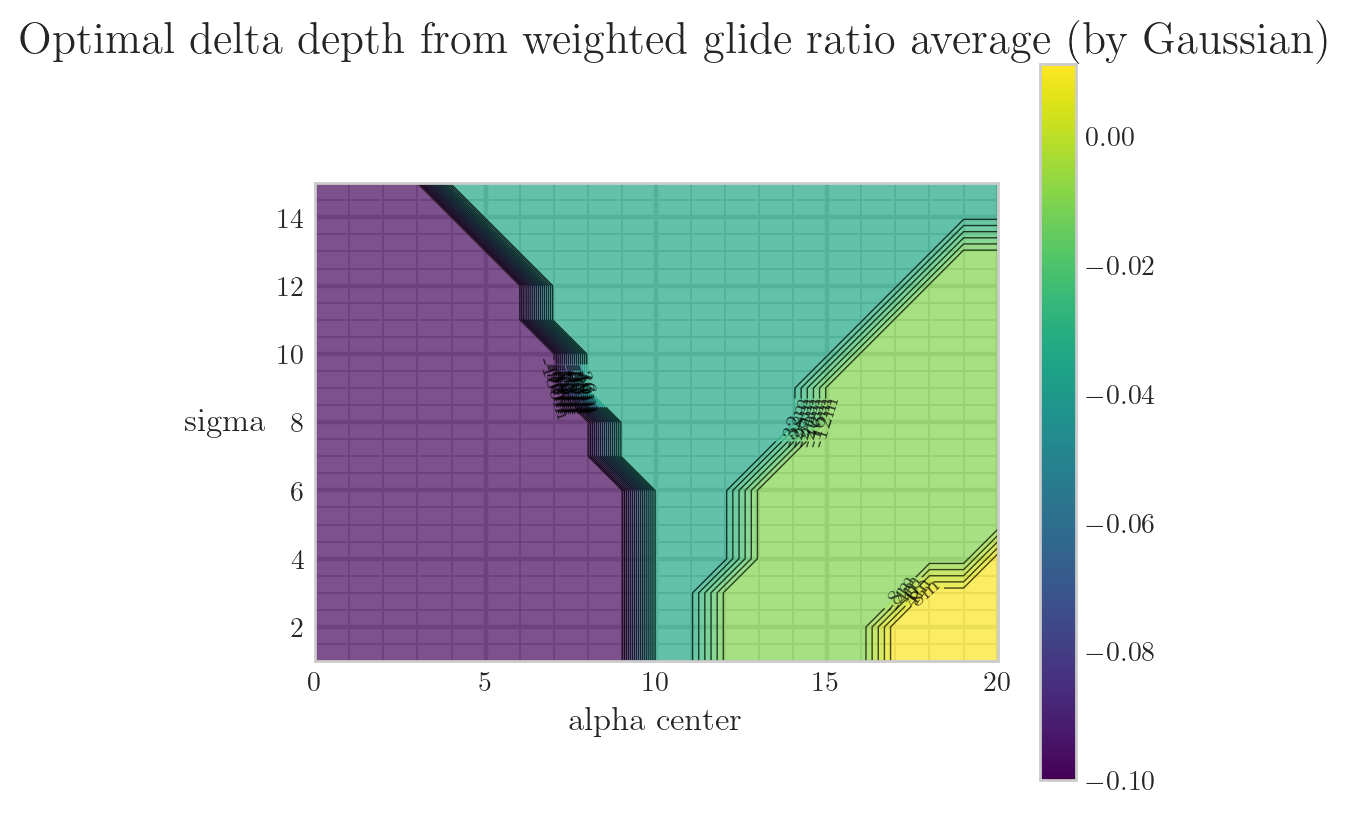
\includegraphics[width=\linewidth]{Pics/04 -Etudes complémentaires/sk5 vb guassian depth.png}
        \caption{$\delta$ cambrure selon les paramètres de la Gaussienne}
        \label{fig:cambrure gaussien sk5 vb}
    \end{subfigure}
    \caption{sk5 vb VB - Sensibilité des résultats 3D en fonction de l'écart-type $\sigma$ et de la valeur centrale $\alpha_{center}$ de la Gaussienne}
    \label{fig:gaussian sensibility sk5 vb}
\end{figure}

\begin{figure}[H]
    \centering
    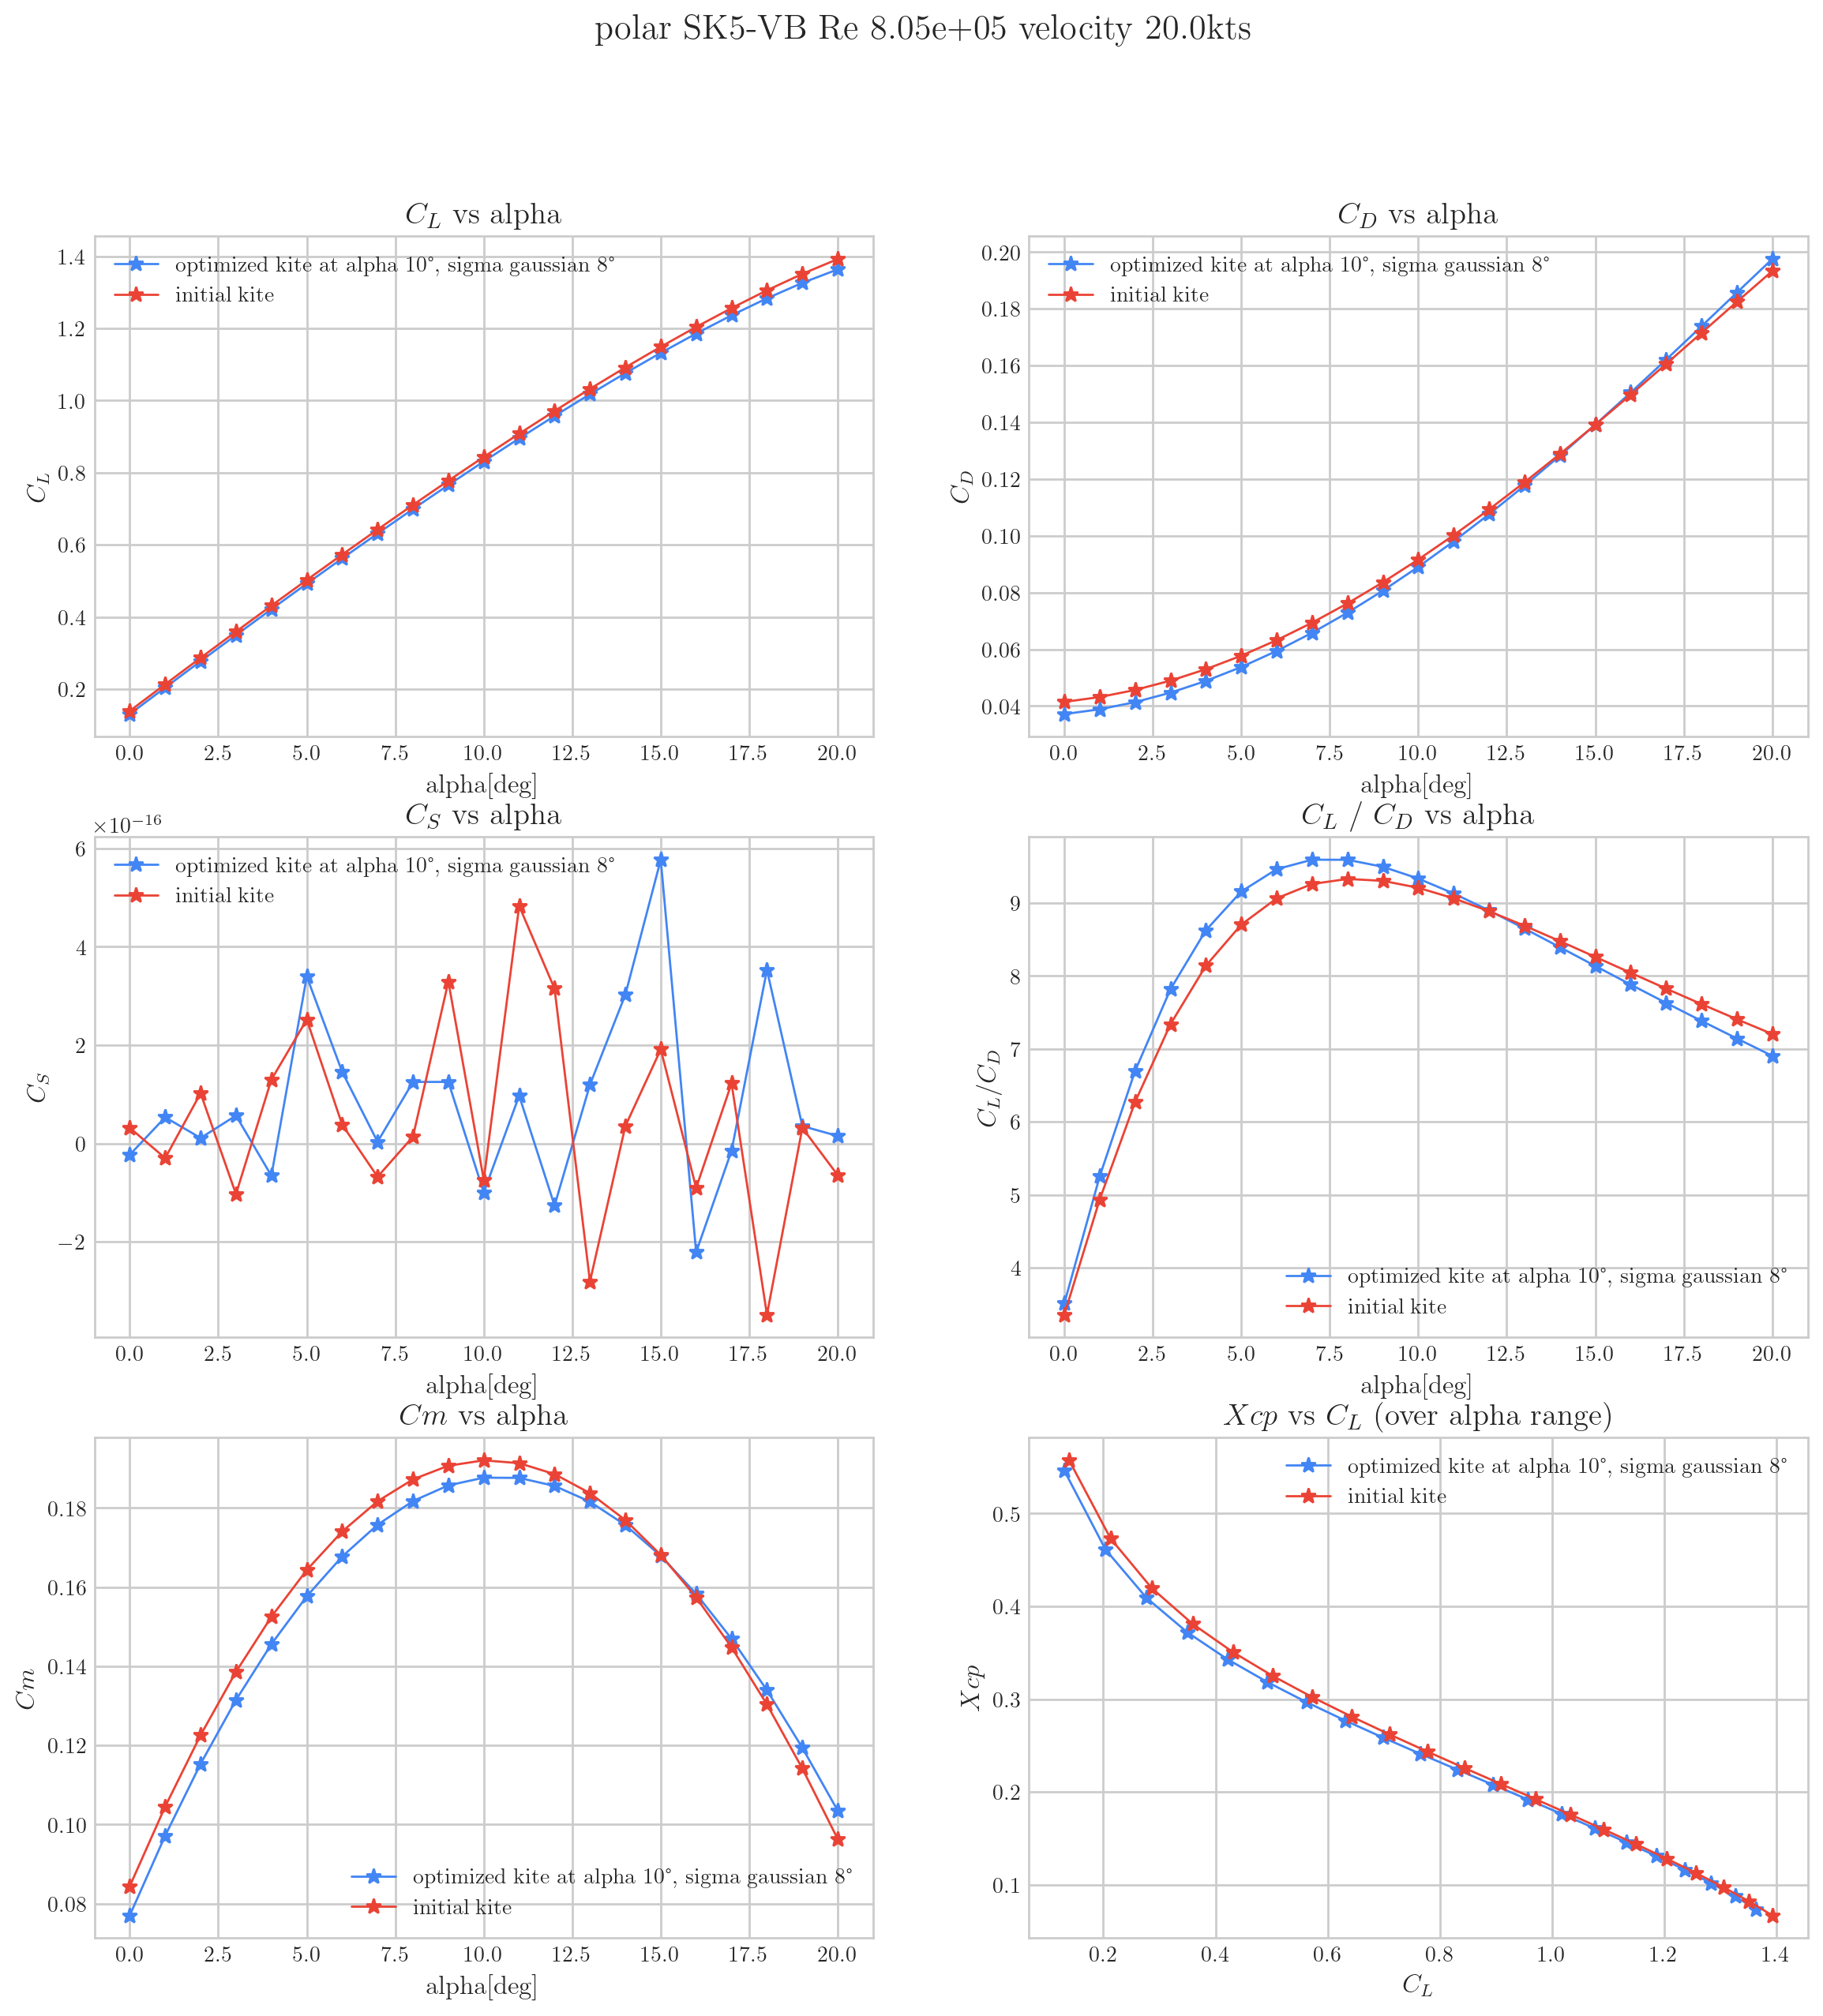
\includegraphics[width=\textwidth]{Pics/04 -Etudes complémentaires/sk5 vb polar.png}
    \caption{Polaire de comparaison}
    \label{fig:polar sk5 vb}
\end{figure}

\textbf{Pour le prochain prototype de SK5 (12/2024)} on propose de choisir un ($\delta t, \delta k)$ qui permette d'optimiser la polaire autour de $\alpha = 15$°

Cela correspond à \textbf{($\delta t, \delta k)$ = (-0.0067, -0.0111)} et une répartition en envergure :
\begin{itemize}
    \item t : 0.0866 0.0845 0.0838 0.0821 0.0800 0.0781 0.0767  0.0760  0.0759 0.0760  0.0767  0.0781 0.0800 0.0821 0.0838 0.0845 0.0866
    \item k : 0.0433 0.0423 0.0534 0.0575 0.0611 0.0641 0.0689 0.0689 0.0689 0.0689 0.0689 0.0641 0.0611 0.0575 0.0534 0.0423 0.0433
\end{itemize}

A comparer avec le kite initial:
\begin{itemize}
    \item t : 0.0849 0.0912 0.0905 0.0888 0.0867 0.0847
    0.0834 0.0826 0.0826 0.0826 0.0834 0.0847
    0.0867 0.0888 0.0905 0.0912 0.0849
    \item k : 0.0425 0.0500 0.0645 0.0686 0.0722 0.0752 0.08 0.08 0.08 0.08 0.08 0.0752 0.0722 0.0686 0.0645 0.0500 0.0425
\end{itemize}

\textbf{La polaire associée est présente sur la figure \ref{fig:polar sk5 vb}}

\textbf{Si on trace l'évolution de ($\delta t_{opti}$, $\delta k_{opti}$) en fonction de $\alpha$ sans moyenner par une Gaussienne} :\\

\begin{figure}[H]
    \centering
    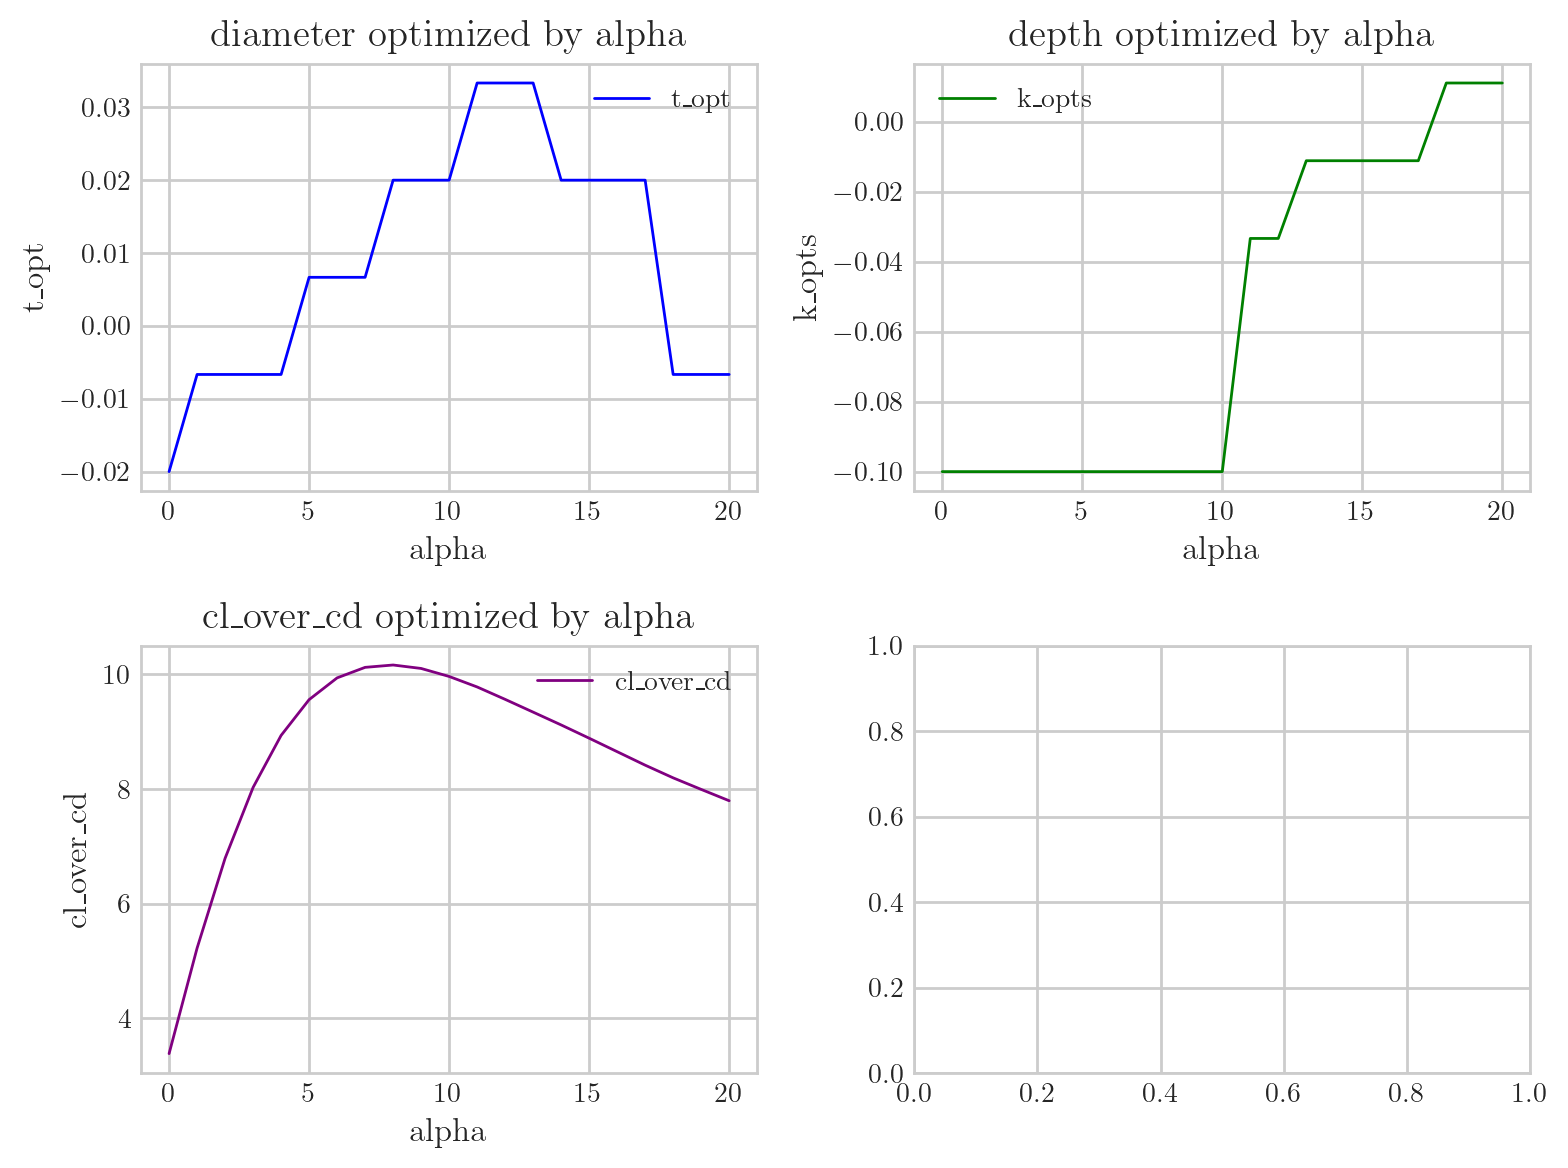
\includegraphics[width=\textwidth]{Pics/04 -Etudes complémentaires/diam deth alpha sk5 vb.png}
    \caption{Evolution de ($\delta t_{opti}$, $\delta k_{opti}$) en fonction de alpha}
    \label{fig:diam depth alpha sk5 vb}
\end{figure}

\begin{figure}[H]
    \centering
    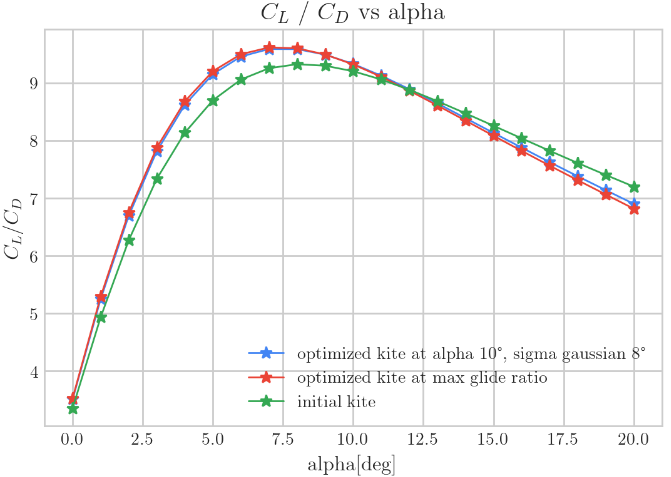
\includegraphics[width=\textwidth]{Pics/04 -Etudes complémentaires/diam deth 2 alpha sk5 vb.png}
    \caption{Evolution de ($\delta t_{opti}$, $\delta k_{opti}$) en fonction de alpha}
    \label{fig:diam depth 2 alpha sk5 vb}
\end{figure}